\chapter{Evaluación del sistema}

Para la evaluación del transmisor, nos pusimos como objetivo final lograr la transmision exitosa hacia un televisor comercial homologado por el LATU. En ese camino, nos propusimos una serie de objetivos de mas corto alcance. Desarrollamos en este capitulo los resultados de las pruebas realizadas con gr-isdbt-tx.

Primero, nos habíamos propuesto lograr la decodificación con gr-isdbt dentro del mismo flowgraph (Eso es, una prueba del sistema punta a punta trasmitiendo en condiciones ideales). Luego, nos propusimos una situación en la que una PC ejecuta el transmisor, enviando la señal a través del USRP, y otra computadora hace lo propio con el receptor gr-isdbt. Esto le agrega a la prueba anterior, el desafío de la puesta en el aire y decodificación de la señal ruidosa.

Finalmente, nos planteamos el objetivo final, la decodificación contra un televisor comercial. En este capitulo desarrollamos estas pruebas, y el nivel de éxito que alcanzo cada una.

\section{Pruebas sobre gr-isdbt}

Considerando que realizamos la mayoría del desarrollo contrastando los bloques del transmisor contra los de gr-isdbt, no parecería en principio un desafió mayor lograr la decodificacion punta a punta. Pero en si, lo es, y eso es parte de la potencia del desarrollo con código abierto desde el otro lado. 

Como receptor, gr-isdbt esta homologado por LATU, por lo tanto, podemos considerarlo como una simulación de un televisor comercial valida. Es en ese punto en el que comenzamos las pruebas. Dentro de un entorno controlado, el transmisor gr-isdbt-tx conectado a la entrada del receptor gr-isdbt.

Existen varios indicadores de calidad en una transmisión digital, en este caso nos basaremos en dos de ellos que son ampliamente utilizados y proporcionan una medida cuantitativa de la calidad de la señal. A continuación definiremos y el \textit{Bit Error Rate} (BER), y el \textit{Modulation Error Rate} (MER).

\subsection{BER}
El estándar ISDB-T en su etapa de codificación de canal hace uso de una combinación de códigos de Reed-Solomon junto con códigos convolucionales. En recepción se utilizan los decodificadores Viterbi y Reed-Solomon, ambos códigos están orientados a la corrección de errores de bits. Resulta importante cuantificar esos errores que se producen así como conocer la proporción de ellos que se han podido recuperar. Es de interés conocer tanto la cantidad de errores que hay antes del Viterbi, luego del Viterbi (antes del Reed-Solomon) y luego del Reed-Solomon.

Se define la tasa de error de bits (BER) como el cociente entre la cantidad de bits erróneos que se recibieron y la cantidad de bits totales.

Para realizar una medición del BER hay que elegir un intervalo de tiempo determinado sobre el cual se va a promediar. En pruebas de aceptación de equipos comerciales se suelen realizar tests que duran varias horas, mientras que para pruebas de monitoreo los tests suelen ser de algunos minutos.





 

\subsection{MER}
La tasa de error de modulación (MER) es una medida de la suma de todas las interferencias que afectan a una señal de TV digital. Se registra la desviación de los puntos del diagrama de constelación de su posición teórica. Esto da una manera de realizar una evaluación cuantitativa sobre la calidad de la señal. Usualmente el MER se expresa en dB como la tasa logarítmica entre el valor RMS de la amplitud de la señal y el módulo del vector error.


\begin{equation}
MER_{RMS} = 10 \log_{10} \left( \dfrac{\sum_{j = 0}^{N-1} I_{j}^{2}+ Q_{j}^{2}}{\sum_{j = 0}^{N-1}\delta I_{j}^{2}+\delta Q_{j}^{2}} \right )
\end{equation}


Tener un MER alto indica una buena calidad en la señal, para los equipos transmisores comerciales se considera un MER de 35dB como muy bueno. Las señales recibidas en un hogar a través de una antena instalada en el techo tienen un MER que se ubica entre los 20dB y 30dB aproximadamente. 

El MER se puede medir de varias maneras según lo que interese considerar. Es común muy calcular el MER para cada una de las capas por separado, pero también es posible considerar todas las señales incluyendo las portadoras piloto. Tener en cuenta las portadoras piloto para el cálculo del MER puede provocar que el promedio esté un poco por encima del MER de las tres capas por separado.



\subsubsection{Pruebas flowgraph}

En este caso ideal, contenido en un mismo flowgraph y con nula variabilidad de las muestras, el transmisor se comporta de forma perfecta. Si encontramos, algunos problemas de consumo de CPU, seguramente debidos a problemas de optimización del código. 
Pero yendo estrictamente a las señales y a su procesamiento, entendemos que la decodificación correcta por parte de gr-isdbt, constituye un éxito para el transmisor. 

\begin{figure}[!h]
	\centering
	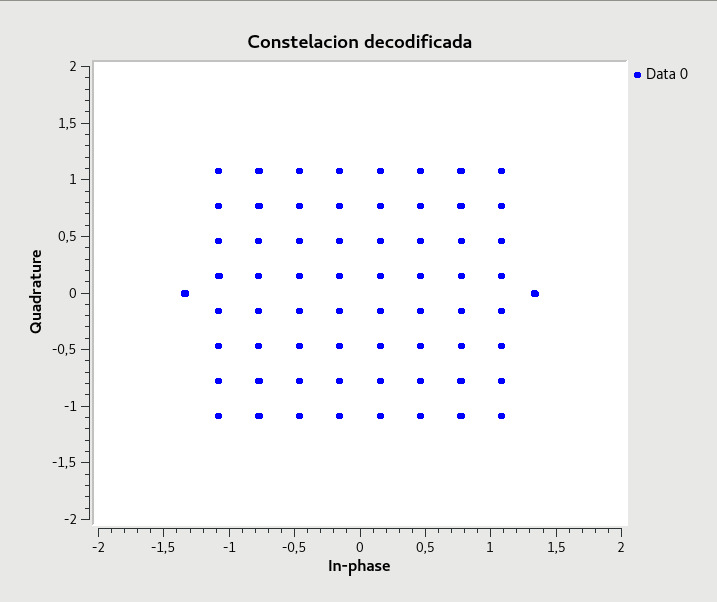
\includegraphics[scale=0.5]{figuras/cap06/const_rec}
	\caption{\label{f:const_rec} Constelación en recepción. Caso ideal.}
\end{figure}

Como se puede ver en la figura \ref{f:const_rec}, el receptor gr-isdbt se sincroniza perfectamente con la señal transmitida, y en la constelación de recepción, vemos la misma constelación que en transmision. Esto no debe sorprender, ya que en esta prueba, el canal esta representado por un cable ideal. 

\subsubsection{Pruebas en el aire}

Realizamos la misma prueba de antes, pero en lugar de simular un canal por un conector ideal del flowgraph de GNU Radio, utilizamos el aire y transmitimos en una linea vista, a través de 10 cm. 

El resultado fue interesante. Si bien no es posible decodificar las señales todavía, intermitentemente es posible observar la constelación en recepción, como se ve en la figura \ref{f:aire}. 

\begin{figure}[!h]
	\centering
	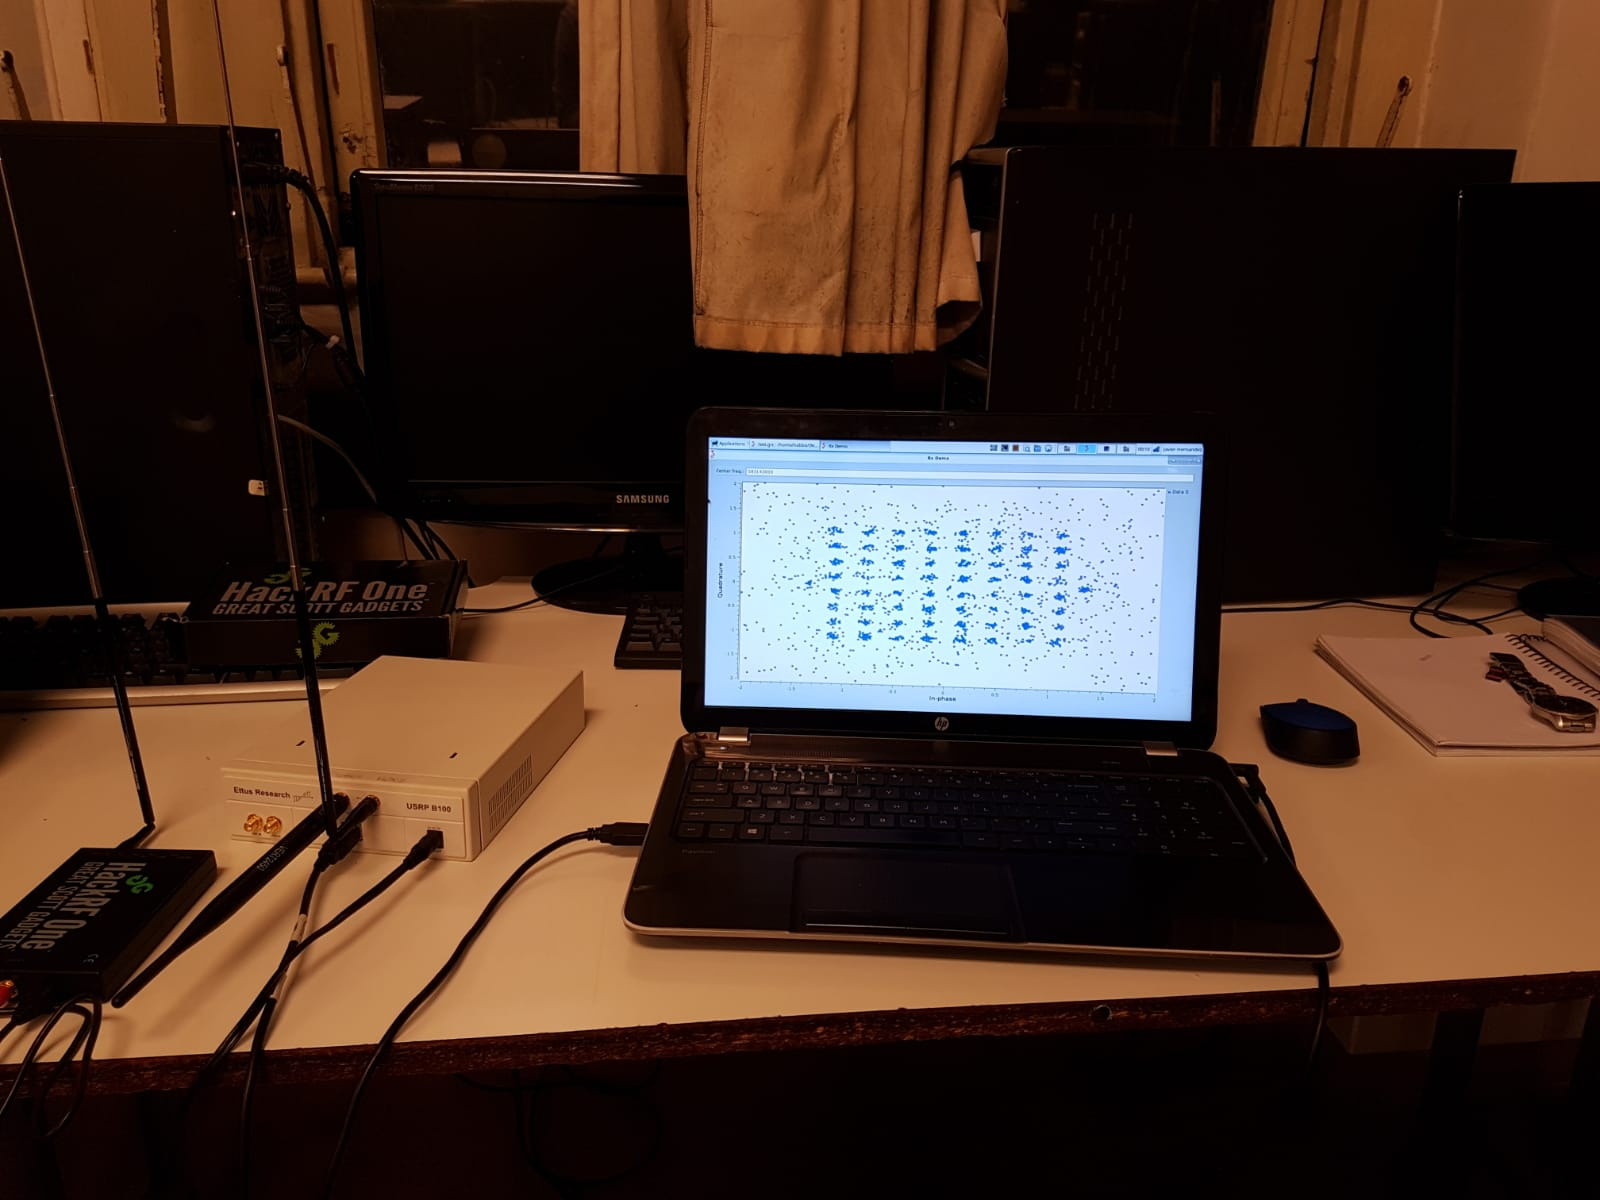
\includegraphics[scale=0.25]{figuras/cap06/aire}
	\caption{\label{f:aire} Constelación en recepción. Por linea vista.}
\end{figure}

Entendemos que tenemos algún problema de sincronismo, surgido seguramente por el uso del USRP. Dado que es el único cambio entre la prueba anterior y esta. 

\section{Pruebas sobre televisores comerciales}

Dado que las pruebas contra gr-isdbt con canal no ideal no fueron exitosas, no pasamos a las pruebas contra un televisor comercial. Hasta no resolver el problema de sincronismo encontrado en la prueba contra gr-isdbt usando el USRP como transmisor, no sera prosible lograr el objetivo planteado al comenzar este proyecto. 